\chapter{Préliminaires}
\label{cp:preliminaires}

Avant de commencer à détailler la stratégie utilisée, il est nécessaire de présenter certaines notions sur lesquelles elle repose.
\section{Structure de données}

Pour représenter la grille du jeu, nous avons décidé d'utiliser une sorte de liste chaînée. Chaque cellule de la grille est représentée par une structure \texttt{Cell} en C, qui contient les informations suivantes :
\begin{enumerate}
    \item Les coordonnées de la cellule dans la grille, représentées par les entiers \texttt{x} et \texttt{y}.
    \item Le nombre de mines adjacentes à la cellule, stocké dans \texttt{adjacentMines}.
    \item Un booléen \texttt{isMine} qui indique si la cellule contient une mine.
    \item Un booléen \texttt{isRevealed} qui indique si la cellule a été révélée.
    \item Un booléen \texttt{isFlagged} qui indique si la cellule a été marquée d'un drapeau.
    \item Un tableau de pointeurs vers les cellules adjacentes, stocké dans \texttt{adjacentCells}.
    \item Un flottant \texttt{probability} qui stocke la probabilité que la cellule contienne une mine.
\end{enumerate}

L'intérêt de stocker les cellules adjacentes dans un tableau de pointeurs est de pouvoir accéder facilement aux cellules voisines d'une cellule donnée. Cela facilite des algorithmes tels que la révélation des cellules adjacentes à une cellule vide, ou le calcul du nombre de mines adjacentes à une cellule donnée.
\newline
\newline
La structure \texttt{Cell} est définie en C comme suit :

\begin{longlisting}
    \begin{minted}{c}
        typedef struct Cell {
            int x;
            int y;
            int adjacentMines;
            bool isMine;
            bool isRevealed;
            bool isFlagged;
            struct Cell** adjacentCells;
            float probability;
        } Cell;
    \end{minted}
    \caption{Structure \texttt{Cell} en C.}
    \label{listing:c-path}
\end{longlisting}
\section{Cellules adjacentes}
\label{sec:cellules-adjacentes}

Dans un jeu de type démineur, une cellule peut avoir jusqu'à huit cellules adjacentes. Ces cellules sont celles qui partagent un côté ou un coin avec la cellule en question. Voici une illustration des cellules adjacentes pour une cellule située au centre d'une grille 3x3 :

\begin{figure}[!htpb]
    \centering
    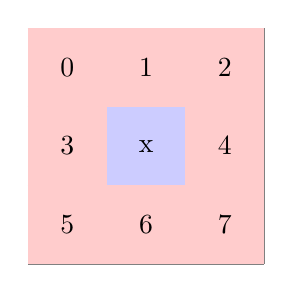
\begin{tikzpicture}
        \draw[step=1cm,gray,very thin] (0,0) grid (3,3);
        \fill[blue!20] (1,1) rectangle (2,2);
        \fill[red!20] (0,0) rectangle (1,1);
        \fill[red!20] (1,0) rectangle (2,1);
        \fill[red!20] (2,0) rectangle (3,1);
        \fill[red!20] (0,1) rectangle (1,2);
        \fill[red!20] (2,1) rectangle (3,2);
        \fill[red!20] (0,2) rectangle (1,3);
        \fill[red!20] (1,2) rectangle (2,3);
        \fill[red!20] (2,2) rectangle (3,3);
        
        \node at (1.5, 1.5) {x}; % Cellule centrale
        \node at (0.5, 0.5) {5}; % En haut à gauche
        \node at (1.5, 0.5) {6}; % En haut
        \node at (2.5, 0.5) {7}; % En haut à droite
        \node at (0.5, 1.5) {3}; % À gauche
        \node at (2.5, 1.5) {4}; % À droite
        \node at (0.5, 2.5) {0}; % En bas à gauche
        \node at (1.5, 2.5) {1}; % En bas
        \node at (2.5, 2.5) {2}; % En bas à droite
    \end{tikzpicture}
    \caption{Illustration des cellules adjacentes dans une grille 3x3. La cellule centrale est en bleu et les cellules adjacentes sont en rouge.}
    \label{fig:cellules-adjacentes}
\end{figure}

Pour déterminer les cellules adjacentes d'une cellule située à la position $(i, j)$ dans une grille, on peut utiliser les décalages suivants :

\begin{itemize}
    \item $(i-1, j-1)$ : en haut à gauche
    \item $(i-1, j)$ : en haut
    \item $(i-1, j+1)$ : en haut à droite
    \item $(i, j-1)$ : à gauche
    \item $(i, j+1)$ : à droite
    \item $(i+1, j-1)$ : en bas à gauche
    \item $(i+1, j)$ : en bas
    \item $(i+1, j+1)$ : en bas à droite
\end{itemize}

Ces décalages permettent de parcourir toutes les cellules adjacentes à une cellule donnée dans la grille.
